% =====================================================================
%  Sentinel-RX: Security-Aware Agentic Recovery of Failing Systems
%  Technical Report -- Humain Hackathon, Challenge 1
%  Single self-contained LaTeX source (pdfLaTeX). No external .bib / .sty.
%  Figures: docs/technical_report/figures/*.png (copied from docs/figures by make report)
%  Every number in this document comes from results/*.json, results/summary.md,
%  docs/RESULTS.md, models/beacon_metrics.json or results/demo_live_trace.json.
% =====================================================================
\documentclass[11pt,a4paper]{article}

% ---------- encoding, fonts ------------------------------------------
\usepackage[T1]{fontenc}
\usepackage[utf8]{inputenc}
\usepackage{lmodern}
\usepackage{microtype}
\usepackage[table,dvipsnames]{xcolor}
\usepackage{amsmath,amssymb}
\usepackage{XCharter}
\usepackage[xcharter,vvarbb]{newtxmath}

% ---------- layout ---------------------------------------------------
\usepackage[a4paper,margin=2.5cm]{geometry}
\usepackage{graphicx}
\usepackage{adjustbox}
\graphicspath{{figures/}}
\usepackage{booktabs}
\usepackage{tabularx}
\usepackage{array}
\usepackage{siunitx}
\usepackage{algorithm}
\usepackage{algpseudocode}
\usepackage{enumitem}
\usepackage{caption}
\usepackage{subcaption}
\usepackage{float}
\usepackage[section]{placeins}
\usepackage{titlesec}
\usepackage{fancyhdr}
\usepackage[skins,breakable]{tcolorbox}
\usepackage{tikz}
\usetikzlibrary{arrows.meta,positioning,shapes.geometric,fit,backgrounds,calc,decorations.pathreplacing}
\usepackage{hyperref}
\usepackage{cleveref}

% ---------- palette --------------------------------------------------
\definecolor{accent}{HTML}{1F3A5F}     % navy
\definecolor{accent2}{HTML}{3C6E9F}    % lighter navy for rules
\definecolor{groupfill}{HTML}{E8F0FA}  % light blue group fill
\definecolor{outfill}{HTML}{FFF4CC}    % soft yellow outputs / evidence
\definecolor{detfill}{HTML}{E4F2EC}    % mint, detectors
\definecolor{llmfill}{HTML}{F1E8F7}    % lavender, LLM
\definecolor{safefill}{HTML}{FDEBD0}   % peach, safety
\definecolor{keyfill}{HTML}{F4F7FB}
\definecolor{limfill}{HTML}{FBF1F1}
\definecolor{decfill}{HTML}{F3F8F3}
\colorlet{attack}{red!75!black}
\definecolor{recovered}{HTML}{2E7D32}
\definecolor{muted}{HTML}{6B7280}

\hypersetup{colorlinks=true,linkcolor=accent,citecolor=accent2,urlcolor=accent2,
  pdftitle={Sentinel-RX: Technical Brief},
  pdfauthor={Abdulrahman Alharbi}}

\sisetup{group-separator={\,},group-minimum-digits=4,detect-weight=true}
\captionsetup{font=small,labelfont={bf,color=accent},skip=6pt}
\setlist{nosep,leftmargin=*}

% ---------- headings -------------------------------------------------
\titleformat{\section}{\color{accent}\Large\bfseries}{\thesection}{0.8em}{}[{\color{accent2!50}\titlerule[0.6pt]}]
\titleformat{\subsection}{\color{accent}\large\bfseries}{\thesubsection}{0.8em}{}
\titleformat{\subsubsection}{\color{accent}\normalsize\bfseries}{\thesubsubsection}{0.8em}{}
\titlespacing*{\section}{0pt}{18pt}{8pt}
\titlespacing*{\subsection}{0pt}{12pt}{5pt}

% ---------- header / footer ------------------------------------------
\pagestyle{fancy}
\fancyhf{}
\fancyhead[L]{\small\color{muted}Sentinel-RX \textemdash\ Technical Report}
\fancyhead[R]{\small\color{muted}\thepage}
\renewcommand{\headrulewidth}{0.4pt}
\renewcommand{\headrule}{\color{accent2!50}\hrule width\headwidth height\headrulewidth}
\fancypagestyle{plain}{\fancyhf{}\renewcommand{\headrulewidth}{0pt}}

% ---------- boxes ----------------------------------------------------
\newtcolorbox{keyfinding}[1]{enhanced,breakable,colback=keyfill,colframe=accent,
  boxrule=0.6pt,arc=2pt,left=6pt,right=6pt,top=4pt,bottom=4pt,
  fonttitle=\bfseries\small,coltitle=white,colbacktitle=accent,title={Key finding \textemdash\ #1}}
\newtcolorbox{designdecision}[1]{enhanced,breakable,colback=decfill,colframe=recovered!70!black,
  boxrule=0.6pt,arc=2pt,left=6pt,right=6pt,top=4pt,bottom=4pt,
  fonttitle=\bfseries\small,coltitle=white,colbacktitle=recovered!70!black,title={Design decision \textemdash\ #1}}
\newtcolorbox{limitation}[1]{enhanced,breakable,colback=limfill,colframe=attack,
  boxrule=0.6pt,arc=2pt,left=6pt,right=6pt,top=4pt,bottom=4pt,
  fonttitle=\bfseries\small,coltitle=white,colbacktitle=attack,title={Limitation \textemdash\ #1}}
\newtcolorbox{summarybox}{enhanced,colback=groupfill,colframe=accent,boxrule=0.8pt,arc=3pt,
  left=8pt,right=8pt,top=6pt,bottom=6pt}

% ---------- tikz visual language -------------------------------------
\tikzset{
  box/.style={draw=accent,fill=white,rounded corners=3pt,align=center,font=\footnotesize,
              minimum height=7mm,inner sep=4pt,line width=0.6pt},
  service/.style={box,fill=groupfill,minimum width=17mm},
  detector/.style={box,fill=detfill},
  llm/.style={box,fill=llmfill},
  safety/.style={box,fill=safefill},
  output/.style={box,fill=outfill},
  good/.style={box,fill=recovered!12,draw=recovered!70!black},
  bad/.style={box,fill=attack!8,draw=attack},
  flow/.style={-{Stealth[length=2.2mm]},line width=0.7pt,draw=accent!85!black},
  beacon/.style={-{Stealth[length=2.2mm]},line width=0.9pt,draw=attack,dashed},
  lbl/.style={font=\tiny,text=muted,fill=white,inner sep=1.5pt,align=center},
  group/.style={draw=accent!55,dashed,rounded corners=6pt,fill=groupfill!45,inner sep=9pt},
  grouplbl/.style={font=\scriptsize\bfseries,text=accent,anchor=south west,inner sep=2pt},
  decision/.style={diamond,aspect=2.4,draw=accent,fill=white,align=center,font=\footnotesize,
                   inner sep=1.5pt,line width=0.6pt},
  brace/.style={decorate,decoration={brace,amplitude=4pt},draw=accent2},
}

\newcommand{\code}[1]{\texttt{#1}}
\newcommand{\pct}[1]{#1\,\%}
\newcommand{\ci}[2]{{\footnotesize[#1,\,#2]}}

\begin{document}
\pagestyle{fancy}
\fancyhead[L]{\small\color{muted}Sentinel-RX \textemdash\ Brief}

% ---------- compact title block ----------
\noindent{\color{accent}\rule{\textwidth}{1.2pt}}\\[0.8em]
{\color{accent}\LARGE\bfseries Sentinel-RX: Security-Aware Agentic Recovery of Failing Systems}\\[0.35em]
{\large Technical brief \textemdash\ Humain Hackathon, Challenge~1: Agentic Recovery of a Failing System}\\[0.35em]
{\normalsize Abdulrahman Alharbi \quad\textperiodcentered\quad 30 October 2026}\\[0.2em]
{\small\color{muted}Companion to the full technical report, \code{sentinel\_rx\_technical\_report.pdf} in the same folder.}\\[0.4em]
{\color{accent}\rule{\textwidth}{1.2pt}}

\vspace{0.8em}
\begin{summarybox}
\small\textbf{In one paragraph.} Sentinel-RX is an agent that identifies, diagnoses, recovers and
\emph{verifies} the recovery of a failing enterprise system when several faults are active at once
and a security compromise may be hiding inside the operational incident. Deterministic detectors
compress telemetry into ranked evidence, a local 7B model reasons over it in a budgeted loop, a
safety layer keeps the actions harmless, and a verification gate refuses to say ``recovered''
until the telemetry agrees. On 20 held-out incidents it recovers \pct{100} of systems with \pct{0}
false claims and zero harmful actions, where a rule-based runbook recovers \pct{45} and a single-shot
LLM falsely claims success \pct{70} of the time. Everything runs on one laptop, free, with no
cloud and no Docker, and every number replays from a committed cache without a model installed.
\end{summarybox}

% =====================================================================
\section{Why this matters}
% =====================================================================

\paragraph{The operational problem.} Incident response is the most expensive, least automated part
of running software. Today's auto-remediation is a runbook: if a threshold fires, run an action.
Runbooks cannot tell a symptom from its cause in a dependency graph, cannot handle two faults at
once, and cannot tell whether what they did worked. LLM agents promise to close that gap, but the
published benchmarks inject one accidental fault per scenario and the best agents resolve roughly
\pct{11} of realistic SRE tasks~\cite{itbench,openrca}.

\paragraph{The security problem.} Some ``performance incidents'' are intrusions. A compromised host
phoning home to a command-and-control server looks, to an ops tool, like a slightly slow service.
If an agent restarts it, the forensic evidence is gone and the implant comes back. No AIOps
benchmark tests whether an agent recognises this or orders its actions correctly (contain, then
eradicate). Sentinel-RX does both, and the benchmark measures it.

\paragraph{The trust problem.} An agent that says ``recovered'' is believed, and the incident is
closed. A false claim is worse than no agent. Sentinel-RX treats its own claim as something to be
verified against telemetry, and the benchmark reports false recovery as a headline metric.

\paragraph{What is useful about it.}
\begin{itemize}
  \item \textbf{A design that degrades safely.} Honesty and harmlessness live in the detectors,
        the safety layer and the verifier, not in the model. Swapping the 7B model for a 1.5B one
        halves recovery but keeps \pct{0} false claims and zero harmful actions: a weaker planner
        becomes an honest escalator, not a confident liar.
  \item \textbf{A benchmark others can reuse.} Multi-fault scenarios with disjoint held-out
        combinations, hidden security faults, perturbations, sanity-floor baselines, ablations,
        bootstrap CIs, a split guard that refuses to run held-out without \code{--final}, and a replay
        cache. It is small, but the \emph{design} transfers to any environment.
  \item \textbf{Cheap.} \num{6103} tokens and 4.6 model calls per incident on a laptop-hosted
        model; the same loop reading raw telemetry needs $5.7\times$ more tokens to recover
        $2.9\times$ fewer incidents.
  \item \textbf{Real processes, same code.} The agent that scores the benchmark also recovers a
        live three-fault incident on five real local processes, byte-identical.
\end{itemize}

% =====================================================================
\section{How it maps to the judging criteria}
% =====================================================================

\begin{table}[H]
\centering\footnotesize
\renewcommand{\arraystretch}{1.15}
\begin{tabularx}{\textwidth}{>{\bfseries\color{accent}}p{3.1cm} X}
\toprule
criterion & evidence (every number is from \code{results/}, held-out split unless stated) \\
\midrule
Task performance & 20 held-out scenarios never used in development, 3 seeds ($n=60$): top-1 root cause \pct{92} [83, 98], per-fault recall \pct{82}, recovered \pct{100} [100, 100], false ``recovered'' \pct{0}, harmful actions 0.00 per run, action precision \pct{81}. Runbook: \pct{45} recovered. Single-shot LLM: \pct{30} recovered, \pct{70} false claims. Recovery is flat at \pct{100} from one to three concurrent faults (\cref{tab:heldout}). \\
Robustness \& adaptation & Recovery stays \pct{95}--\pct{100} under noisy logs, missing metrics, renamed services and timestamp jitter; an \emph{unseen} fault type is never named but its service is localized (\pct{94}) and all 8 runs recover; a 1.5B model keeps \pct{0} false claims and 0 harm. Same agent runs unchanged on the simulator and on five real processes (\cref{sec:results}). \\
Evaluation \& iteration & Four dev iterations with before/after numbers (top-1 70 $\to$ 90\,\%, recovered 73 $\to$ 100\,\%, calls 7.4 $\to$ 4.0); a mid-development \emph{scorer audit} that found two lenient spots, fixed them and re-scored every earlier run; do-nothing and random sanity floors (\pct{0} recovered); four ablations that locate each guarantee in one component; 109 tests; CI that replays every held-out result (\cref{sec:honest}). \\
Technical judgment \& creativity & Hybrid design (detectors compress, LLM integrates) measured against its raw-telemetry twin; a RandomForest beacon detector on scale-invariant timing features with destination knowledge as a prior (AP 0.999, 0 false positives on health checks and update polls); contain-before-restart ordering; transactional rollback; a verification gate with a remembered healthy baseline and a known-beacon rule; health $=\tfrac12\overline{h}+\tfrac12\min h$ so one sick service cannot hide (\cref{sec:design}). \\
Engineering quality & One \code{make} target per step; pinned dependencies; typed, ruff-clean modules; one \code{Env} interface for simulator and live system; content-addressed LLM cache, and CI replays every committed held-out result and diffs it run by run, with no model; one git branch per phase merged with \code{--no-ff}; a run log with git revision for every held-out run (\cref{sec:repro}). \\
Communication & README with real console output, a static site with leaderboard, charts and an incident replay viewer, DESIGN / RESULTS / LIMITATIONS documents, a literature review with a gap analysis the design answers point by point, the full technical report, and this brief. \\
\bottomrule
\end{tabularx}
\end{table}

% =====================================================================
\section{What it is}
\label{sec:design}
% =====================================================================

\Cref{fig:arch} shows the system. The agent talks to an environment only through a small
interface (status, metrics, logs, flows, eight allow-listed actions); it never sees the
simulator's fault list. Four deterministic detectors turn thousands of records into a short ranked
evidence list: robust z-scores against a remembered healthy baseline, log-template signatures, a
dependency-aware ranker that discounts upstream symptoms explained by a sick dependency (the single
biggest win over threshold runbooks), and a RandomForest beacon detector on scale-invariant
inter-arrival features. The LLM (\code{qwen2.5:7b} via Ollama, two JSON calls per iteration)
proposes ranked hypotheses and up to three targeted checks, then an ordered plan. The safety
layer enforces the allowlist, refuses containment of hosts without beacon evidence, reorders plans
so containment precedes restarts, and undoes any action that drops observable health by more than
0.15. The verification gate compares post-action telemetry with the healthy baseline and re-scores
known beacon pairs; the agent may claim ``recovered'' only when nothing is flagged, otherwise it
loops (budget 8) or escalates with the trace.

\begin{designdecision}{why hybrid, why a 7B model, why no Docker}
The LLM is good at integrating heterogeneous evidence and ordering a plan, bad at scanning four
thousand flow records. Giving it ranked evidence instead of raw telemetry is both the cheapest and
the most accurate configuration tested (\cref{tab:heldout}). A locally hosted 7B model keeps the
whole system free and private, and its weaknesses (mixing facts between services, ignoring status
fields) were handled with per-service evidence grouping and a repeated-plan guard rather than a
bigger model. Five stdlib processes boot in a second and need no container runtime, which the brief
forbade anyway.
\end{designdecision}

\begin{figure}[H]
\centering
\adjustbox{max width=0.8\textwidth}{%
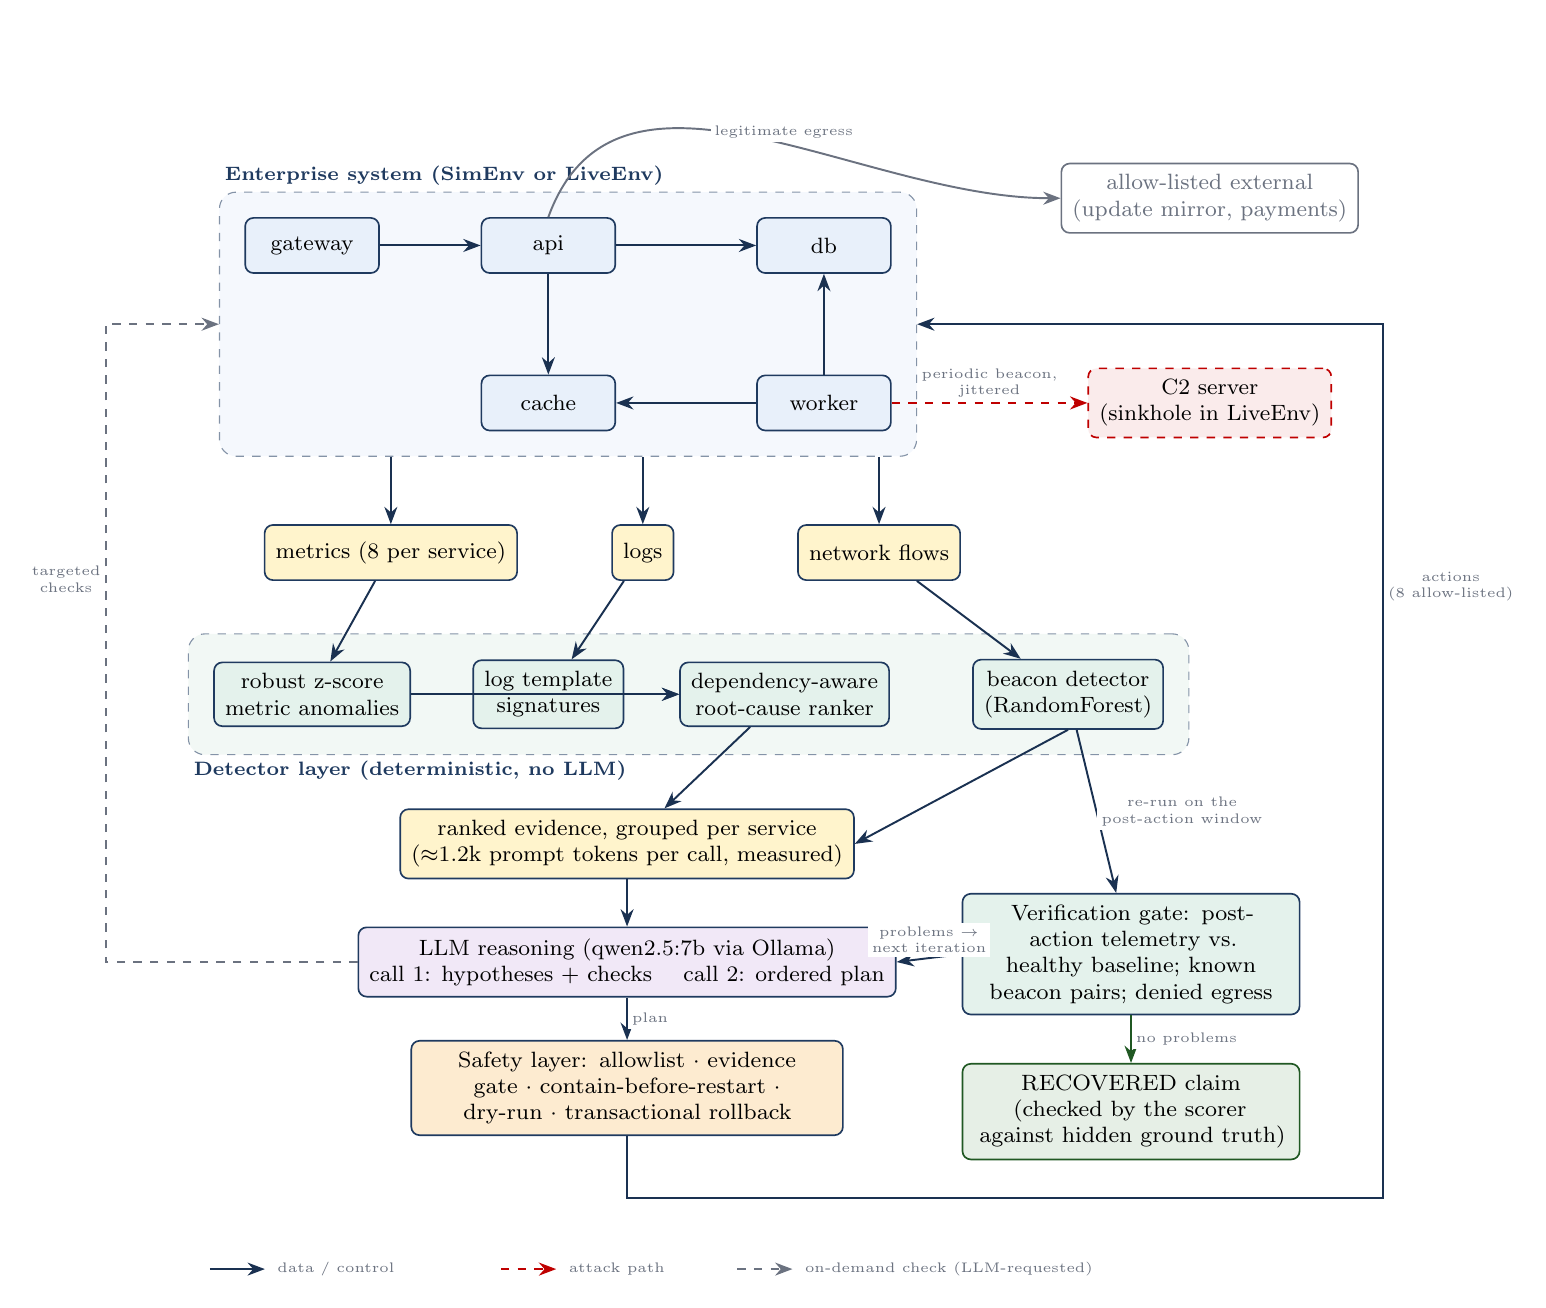
\begin{tikzpicture}
  % ---- enterprise system ----
  \node[service] (gw) at (0,2) {gateway};
  \node[service] (api) at (3,2) {api};
  \node[service] (db) at (6.5,2) {db};
  \node[service] (cache) at (3,0) {cache};
  \node[service] (worker) at (6.5,0) {worker};
  \draw[flow] (gw) -- (api);
  \draw[flow] (api) -- (db);
  \draw[flow] (api) -- (cache);
  \draw[flow] (worker) -- (db);
  \draw[flow] (worker) -- (cache);
  \begin{scope}[on background layer]
    \node[group,fit=(gw)(api)(db)(cache)(worker),
          label={[grouplbl]north west:Enterprise system (SimEnv or LiveEnv)}] (sys) {};
  \end{scope}
  % ---- outside world ----
  \node[bad,dashed] (c2) at (11.4,0) {C2 server\\(sinkhole in LiveEnv)};
  \draw[beacon] (worker) -- node[lbl,above] {periodic beacon,\\jittered} (c2);
  \node[box,draw=muted,text=muted] (ext) at (11.4,2.6) {allow-listed external\\(update mirror, payments)};
  \draw[flow,draw=muted] (api.north) to[out=70,in=180] node[lbl,above,pos=0.55] {legitimate egress} (ext.west);
  % ---- telemetry ----
  \node[output] (met) at (1,-1.9) {metrics (8 per service)};
  \node[output] (logs) at (4.2,-1.9) {logs};
  \node[output] (flows) at (7.2,-1.9) {network flows};
  \draw[flow] (sys.south -| met) -- (met);
  \draw[flow] (sys.south -| logs) -- (logs);
  \draw[flow] (sys.south -| flows) -- (flows);
  % ---- detectors ----
  \node[detector] (zs) at (0,-3.7) {robust z-score\\metric anomalies};
  \node[detector] (lt) at (3,-3.7) {log template\\signatures};
  \node[detector] (rk) at (6,-3.7) {dependency-aware\\root-cause ranker};
  \node[detector] (bc) at (9.6,-3.7) {beacon detector\\(RandomForest)};
  \draw[flow] (met) -- (zs);
  \draw[flow] (logs) -- (lt);
  \draw[flow] (flows) -- (bc);
  \draw[flow] (zs) -- (rk);
  \draw[flow] (lt) -- (rk);
  \begin{scope}[on background layer]
    \node[group,fill=detfill!50,fit=(zs)(lt)(rk)(bc),
          label={[grouplbl,anchor=north west]south west:Detector layer (deterministic, no LLM)}] (det) {};
  \end{scope}
  % ---- evidence, LLM, safety (left column) ----
  \node[output,minimum width=52mm] (ev) at (4,-5.6) {ranked evidence, grouped per service\\($\approx$1.2k prompt tokens per call, measured)};
  \draw[flow] (rk) -- (ev);
  \draw[flow] (bc.south) -- (ev.east);
  \node[llm,minimum width=52mm] (llm) at (4,-7.1) {LLM reasoning (qwen2.5:7b via Ollama)\\call 1: hypotheses + checks \quad call 2: ordered plan};
  \draw[flow] (ev) -- (llm);
  \draw[flow,dashed,draw=muted] (llm.west) -- ++(-3.2,0) |- node[lbl,pos=0.3,left] {targeted\\checks} (sys.west);
  \node[safety,text width=52mm] (safe) at (4,-8.7) {Safety layer: allowlist $\cdot$ evidence gate $\cdot$ contain-before-restart $\cdot$ dry-run $\cdot$ transactional rollback};
  \draw[flow] (llm) -- node[lbl,right] {plan} (safe);
  % ---- verification (right column) ----
  \node[detector,text width=40mm] (ver) at (10.4,-7.0) {Verification gate: post-action telemetry vs.\ healthy baseline; known beacon pairs; denied egress};
  \draw[flow] (bc) -- node[lbl,right] {re-run on the\\post-action window} (ver);
  \draw[flow] (ver.west) -- node[lbl,above] {problems $\rightarrow$\\next iteration} (llm.east);
  \node[good,text width=40mm] (rec) at (10.4,-9.0) {RECOVERED claim (checked by the scorer against hidden ground truth)};
  \draw[flow,draw=recovered!70!black] (ver) -- node[lbl,right] {no problems} (rec);
  % ---- actions back into the system ----
  \draw[flow] (safe.south) |- (13.6,-10.1) |- node[lbl,pos=0.35,right] {actions\\(8 allow-listed)} (sys.east);
  % ---- legend ----
  \draw[flow] (-1.3,-11.0) -- (-0.6,-11.0); \node[lbl,anchor=west] at (-0.5,-11.0) {data / control};
  \draw[beacon] (2.4,-11.0) -- (3.1,-11.0); \node[lbl,anchor=west] at (3.2,-11.0) {attack path};
  \draw[flow,dashed,draw=muted] (5.4,-11.0) -- (6.1,-11.0); \node[lbl,anchor=west] at (6.2,-11.0) {on-demand check (LLM-requested)};
\end{tikzpicture}}
\caption{System architecture. Telemetry from the enterprise system is compressed by four
deterministic detectors into ranked evidence; the LLM reasons, the safety layer screens and executes,
and the verification gate closes the loop. The beacon path from \code{worker} to the C2 server is
the hidden security incident.}
\label{fig:arch}
\end{figure}


% =====================================================================
\section{Results}
\label{sec:results}
% =====================================================================

\begin{table}[H]
\centering\footnotesize
\caption{Held-out results (\code{qwen2.5:7b}, 20 scenarios, 95\,\% bootstrap CIs; $n$ = runs). Harmful actions are counts per run. Source: \code{results/summary.md}.}
\label{tab:heldout}
\setlength{\tabcolsep}{4pt}
\adjustbox{max width=\textwidth}{%
\begin{tabular}{l r r r r r r r r r}
\toprule
config & top-1 & recall & recovered & false ``rec.'' & harmful / run & action prec. & calls & tokens & $n$ \\
\midrule
\rowcolor{groupfill}\textbf{agent} & \textbf{92} \ci{83}{98} & \textbf{82} \ci{74}{89} & \textbf{100} \ci{100}{100} & \textbf{0} \ci{0}{0} & \textbf{0.00} & \textbf{81} \ci{74}{88} & 4.6 & \num{6103} & 60 \\
runbook & 87 \ci{78}{95} & 81 \ci{74}{87} & 45 \ci{32}{58} & 5 \ci{0}{12} & 0.00 & 74 \ci{68}{80} & 0 & 0 & 60 \\
single\_shot & 63 \ci{50}{75} & 50 \ci{41}{59} & 30 \ci{20}{42} & 70 \ci{58}{80} & 0.27 \ci{0.15}{0.38} & 37 \ci{30}{43} & 1.0 & \num{2421} & 60 \\
llm\_only & 35 \ci{15}{55} & 44 \ci{28}{61} & 35 \ci{15}{55} & 15 \ci{0}{30} & 0.55 \ci{0.15}{1.05} & 25 \ci{13}{39} & 18.4 & \num{35018} & 20 \\
do\_nothing & 0 & 0 & 0 & 0 & 0.00 & n/a & 0 & 0 & 60 \\
random & 0 & 0 & 0 & 10 \ci{3}{18} & 3.45 \ci{2.92}{3.98} & 5 \ci{4}{7} & 0 & 0 & 60 \\
\bottomrule
\end{tabular}}
\end{table}

\begin{figure}[H]
\centering
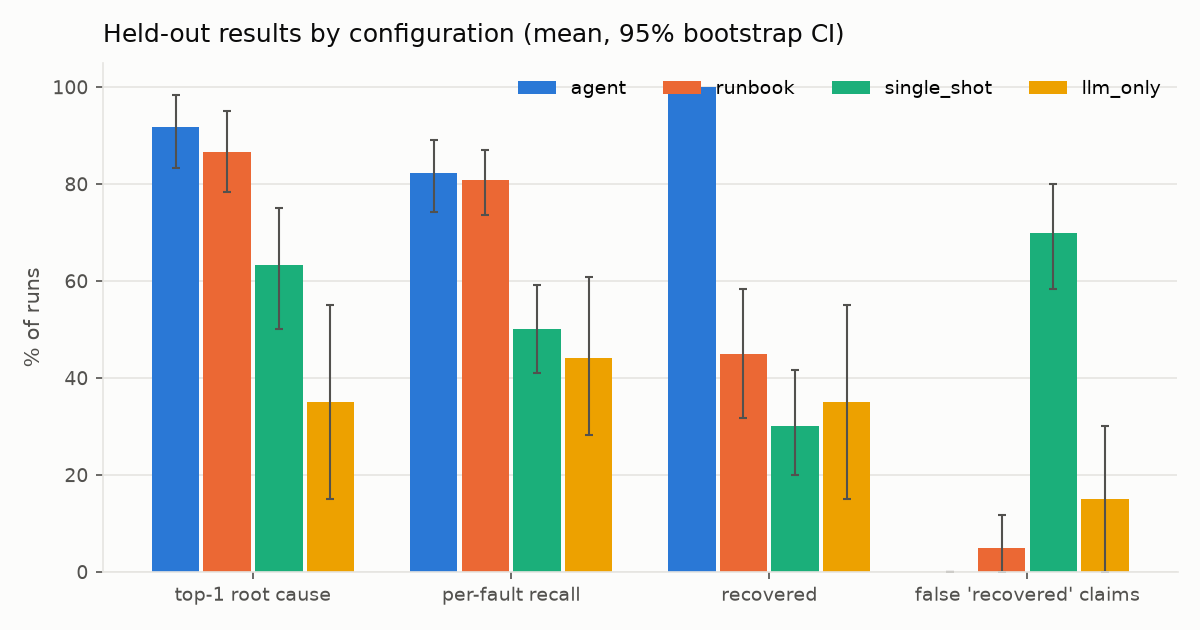
\includegraphics[width=0.88\textwidth]{results-by-config.png}
\caption{Held-out top-1, per-fault recall, recovery and false-recovery rate per configuration, 95\,\% bootstrap CIs.}
\end{figure}

\paragraph{Concurrency.} Recovered / top-1 by number of concurrent faults: agent \pct{100}/\pct{75},
\pct{100}/\pct{93}, \pct{100}/\pct{100} for 1, 2, 3 faults; runbook \pct{75}/\pct{50},
\pct{37}/\pct{93}, \pct{38}/\pct{100}; single\_shot \pct{75}/\pct{50}, \pct{33}/\pct{67},
\pct{0}/\pct{67}. Every baseline degrades with concurrency; the agent does not. Its single-fault top-1
misses are type confusions where the fix coincides (a cache latency injection labelled
\code{cache\_failure}, resolved by a restart), counted as diagnosis misses but not recovery misses.

\paragraph{Security.} In the 27 held-out runs with a security fault (21 with a C2 beacon) the agent recovered \pct{100},
never restarted a compromised host before containing it and never contained an uncompromised one.
single\_shot (27 runs) and llm\_only (9 runs, 1 seed) did so routinely (0.48 and 1.11 harmful actions per run); a random walk over
the same eight actions is harmful 3.04 times per run. The action space is dangerous by default; the
safety layer, not the model, makes it safe.

\begin{table}[H]
\centering\footnotesize
\caption{Robustness (agent, held-out variants, 1 seed) and ablations (held-out, 1 seed, $n=20$; deltas vs.\ the full agent on the same seed).}
\label{tab:robab}
\setlength{\tabcolsep}{4pt}
\begin{tabular}{l r r r r}
\toprule
variant & top-1 & recovered & false ``rec.'' & harmful / run \\
\midrule
\rowcolor{groupfill}full agent, clean held-out (3 seeds, $n=60$) & \pct{92} & \pct{100} & \pct{0} & 0.00 \\
noisy logs (+\pct{80} benign lines) & \pct{95} & \pct{100} & \pct{0} & 0.00 \\
missing metrics & \pct{90} & \pct{95} & \pct{0} & 0.00 \\
renamed services & \pct{90} & \pct{100} & \pct{0} & 0.00 \\
timestamp jitter ($\sigma=2$\,s) & \pct{90} & \pct{100} & \pct{0} & 0.00 \\
unseen fault type (dns\_failure, $n=8$)\textsuperscript{*} & \pct{62} & \pct{100} & \pct{0} & 0.00 \\
smaller model (qwen2.5:1.5b) & \pct{40} & \pct{50} & \pct{0} & 0.00 \\
\midrule
ablation: no verification gate & \pct{80} ($-10$) & \pct{20} ($-80$) & \pct{80} ($+80$) & 0.00 \\
ablation: no loop (one iteration) & \pct{80} ($-10$) & \pct{20} ($-80$) & \pct{0} & 0.00 \\
ablation: no beacon detector & \pct{85} ($-5$) & \pct{50} ($-50$) & \pct{35} ($+35$) & 0.05 \\
ablation: no safety layer & \pct{90} ($0$) & \pct{100} ($0$) & \pct{0} & 0.60 ($+0.60$) \\
\bottomrule
\end{tabular}

\smallskip\raggedright\footnotesize\textsuperscript{*}The unseen type is never named (recall on it 0/8); top-1 here is the known co-fault. Its service is localized in \pct{94} of cases and every run recovers.
\end{table}

\begin{keyfinding}{each component protects a different metric}
Without the verification gate the agent takes the same actions but \emph{claims} success in
\pct{80} of runs; without the loop it recovers only \pct{20} but escalates honestly; without the
beacon detector recovery halves and no security scenario is recovered; without the safety layer
recovery is unchanged but 0.60 harmful actions per run appear. Diagnosis comes mostly from the
detectors (the LLM-free runbook reaches top-1 \pct{87}); recovery from the loop; honesty from the
gate; harmlessness from the safety layer. The model's contribution is integration and planning over
evidence it did not have to find.
\end{keyfinding}

\paragraph{Cost.} Agent: 4.6 calls, \num{6103} tokens, 2.2 iterations and 190\,s of laptop time per
incident. llm\_only: 18.4 calls, \num{35018} tokens, 816\,s. The 1.5B model is not cheaper either
(17.8 calls, \num{29659} tokens) because it loops on wrong plans.

\paragraph{Live demonstration.} \Cref{fig:timeline} is the recorded \code{make demo-live} run on five
real processes: a memory leak on \code{api}, a connection-pool hold on \code{db} and a C2 beacon on
\code{worker} every $\approx$4\,s, injected together after a 35\,s baseline (health 1.00 $\to$ 0.10).
The model's first plan tried to restart \code{worker}; the safety layer blocked it because the beacon
detector had flagged the host. Verification refused ``recovered'' twice, naming the live beacon. In
the third iteration the model blocked \code{worker}'s egress and only then restarted it. Ground truth
from the live system afterwards: no active faults, restart-before-containment $=0$, final health 1.00;
6 LLM calls, \num{9058} tokens.

\begin{figure}[H]
\centering
\adjustbox{max width=\textwidth}{%
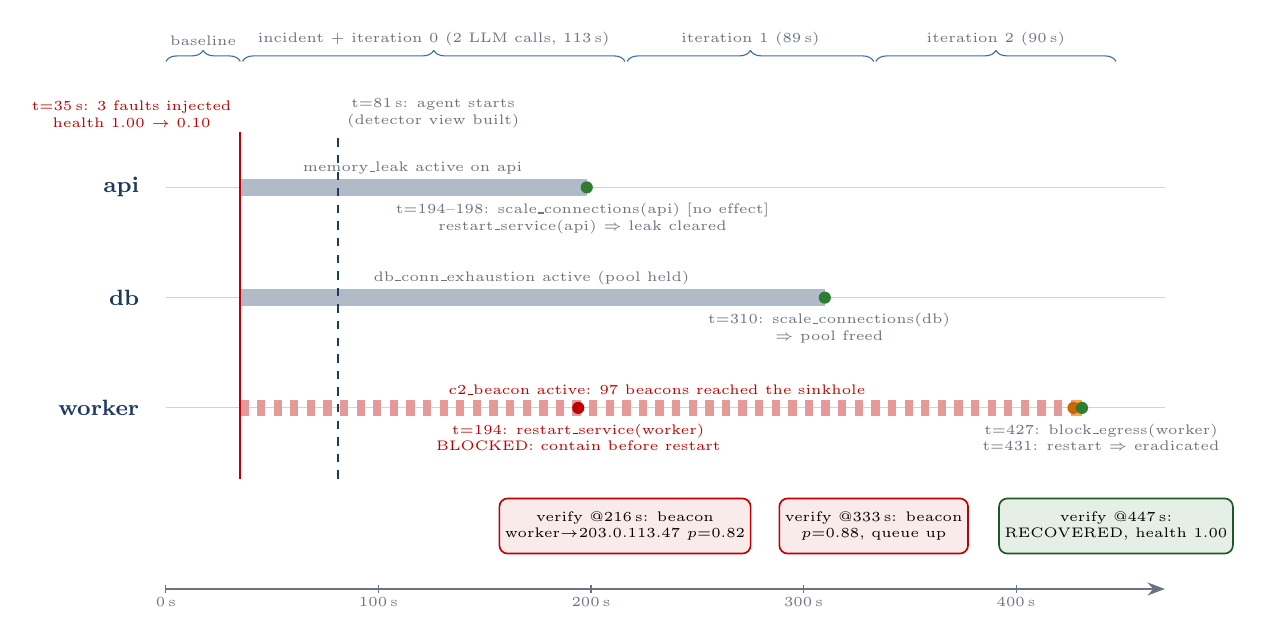
\begin{tikzpicture}[x=0.027cm,y=1cm]
  % lanes
  \foreach \y/\n in {3.4/api,2.0/db,0.6/worker} {
    \node[anchor=east,font=\footnotesize\bfseries,text=accent] at (-8,\y) {\n};
    \draw[gray!35] (0,\y) -- (470,\y);
  }
  % fault bars
  \draw[line width=6pt,accent!35] (35,3.4) -- (198,3.4);
  \node[lbl,above=3pt] at (116,3.4) {memory\_leak active on api};
  \draw[line width=6pt,accent!35] (35,2.0) -- (310,2.0);
  \node[lbl,above=3pt] at (172,2.0) {db\_conn\_exhaustion active (pool held)};
  \draw[line width=6pt,attack!40,dashed] (35,0.6) -- (427,0.6);
  \node[lbl,above=3pt,text=attack] at (231,0.6) {c2\_beacon active: 97 beacons reached the sinkhole};
  \draw[line width=6pt,orange!70] (427,0.6) -- (431,0.6);
  % injection and agent start
  \draw[attack,line width=0.8pt] (35,-0.3) -- (35,4.1);
  \node[lbl,text=attack,anchor=south east] at (33,4.1) {t=35\,s: 3 faults injected\\health 1.00 $\to$ 0.10};
  \draw[accent,line width=0.8pt,dashed] (81,-0.3) -- (81,4.1);
  \node[lbl,anchor=south west] at (83,4.1) {t=81\,s: agent starts\\(detector view built)};
  % actions
  \fill[recovered] (198,3.4) circle (2.2pt);
  \node[lbl,below=4pt] at (196,3.4) {t=194--198: scale\_connections(api) [no effect]\\restart\_service(api) $\Rightarrow$ leak cleared};
  \fill[recovered] (310,2.0) circle (2.2pt);
  \node[lbl,below=4pt] at (312,2.0) {t=310: scale\_connections(db)\\$\Rightarrow$ pool freed};
  \fill[attack] (194,0.6) circle (2.2pt);
  \node[lbl,below=4pt,text=attack] at (194,0.6) {t=194: restart\_service(worker)\\BLOCKED: contain before restart};
  \fill[orange!80!black] (427,0.6) circle (2.2pt);
  \fill[recovered] (431,0.6) circle (2.2pt);
  \node[lbl,below=4pt] at (440,0.6) {t=427: block\_egress(worker)\\t=431: restart $\Rightarrow$ eradicated};
  % verification marks
  \node[bad,font=\tiny,inner sep=2pt] at (216,-0.9) {verify @216\,s: beacon\\worker$\to$203.0.113.47 $p$=0.82};
  \node[bad,font=\tiny,inner sep=2pt] at (333,-0.9) {verify @333\,s: beacon\\$p$=0.88, queue up};
  \node[good,font=\tiny,inner sep=2pt] at (447,-0.9) {verify @447\,s:\\RECOVERED, health 1.00};
  % axis
  \draw[flow,draw=muted] (0,-1.7) -- (470,-1.7);
  \foreach \t in {0,100,200,300,400} { \draw[muted] (\t,-1.75) -- (\t,-1.65); \node[lbl,below] at (\t,-1.75) {\t\,s}; }
  % braces for phases
  \draw[brace] (0,5.0) -- (35,5.0) node[lbl,midway,above=4pt] {baseline};
  \draw[brace] (36,5.0) -- (216,5.0) node[lbl,midway,above=4pt] {incident $+$ iteration 0 (2 LLM calls, 113\,s)};
  \draw[brace] (217,5.0) -- (333,5.0) node[lbl,midway,above=4pt] {iteration 1 (89\,s)};
  \draw[brace] (334,5.0) -- (447,5.0) node[lbl,midway,above=4pt] {iteration 2 (90\,s)};
\end{tikzpicture}}
\caption{The recorded live-demo incident: memory leak on \code{api}, pool exhaustion on \code{db}
and a C2 beacon on \code{worker}, on five real processes. Bars are the hidden fault lifetimes; dots
are the actions that ended them; boxes below the axis are the verifier's verdicts. Times are seconds
since the services started (\code{results/demo\_live\_trace.json}).}
\label{fig:timeline}
\end{figure}

% =====================================================================
\section{How the numbers were kept honest}
\label{sec:honest}
% =====================================================================

\begin{itemize}
  \item \textbf{Split discipline.} 30 dev scenarios for tuning, 20 held-out with fault combinations
        and type multisets never seen in dev and a disjoint seed range; the runner refuses non-dev
        splits without \code{--final} and logs every such run with its git revision. The agent, detectors,
        prompts, simulator and scorer were frozen (tag \code{v1-frozen}) before the first held-out run.
  \item \textbf{Sanity floors.} do\_nothing and random are permanent baselines: any scenario they
        ``recover'' is a broken check. They recover \pct{0} on held-out and \pct{0}--\pct{1} on dev.
  \item \textbf{Scorer audit.} Mid-development the recovery metric was challenged. Tests now prove
        no fault clears on its own or via a wrong action or target. Two lenient spots were
        found and fixed: the observable health formula let one sick service hide behind four healthy
        ones (now $\tfrac12\overline{h}+\tfrac12\min h$), and containment of an uncompromised host was
        not counted as harmful. Re-scoring showed that agent v0 and v1 were \emph{not} harmless
        (0.27 and 0.23 wrong containments per run); the containment gate introduced in v2 removed that.
        Pre-audit numbers are kept, labelled, in \code{docs/RESULTS.md}.
  \item \textbf{Iteration log.} v0 $\to$ v3 on dev: top-1 70 $\to$ 90\,\%, recovered 73 $\to$ 100\,\%,
        false claims 0\,\% throughout, calls 7.4 $\to$ 4.0, each change named with its before/after numbers.
  \item \textbf{Regression checks.} 109 tests; CI runs ruff, the tests, a replay smoke run with
        floors, and replays all 16 committed held-out and perturbation results (508 runs) from the
        cache, failing on any difference.
\end{itemize}

% =====================================================================
\section{Reproduce it}
\label{sec:repro}
% =====================================================================

Python 3.12, no Docker. Replay targets need no model; recording targets need Ollama with
\code{qwen2.5:7b}. Every number in this brief replays from the committed cache.

\begin{tcolorbox}[enhanced,colback=keyfill,colframe=accent!60,boxrule=0.5pt,arc=2pt,left=6pt,right=6pt]
\scriptsize\begin{verbatim}
make setup           # venv, pinned deps, scenarios, beacon detector training (~1 min)
make test            # 109 tests, no LLM needed
make smoke           # 5 dev scenarios from the replay cache, no LLM (< 60 s)
make demo-live       # 5 real local processes + 3 concurrent faults + the agent (needs Ollama)
make all-final       # held-out + perturbations + ablations + report (needs Ollama; hours)
python -m bench.runner --split heldout --config agent --seeds 3 --final --replay   # exact replay
python -m http.server -d site 8000     # leaderboard, charts, incident replay viewer
\end{verbatim}
\end{tcolorbox}

% =====================================================================
\section{Limitations, stated plainly}
% =====================================================================

\begin{limitation}{what this does not show}
The simulator is small and hand-written (five services, nine known fault types with scripted
symptoms that match the taxonomy the agent is told), and the prompt's ``Fix:'' line for each
fault type is generated from the simulator's own accepted remedies, the same knowledge the
runbook baseline hard-codes. The benchmark therefore measures diagnosis under concurrent faults,
safe ordering and verified recovery, not the discovery of new remedies. The unseen fault type is
recovered but never named. Top-1 counts a hit on any injected fault; per-fault recall is stricter. The beacon detector was trained on synthetic timings, not real captures. llm\_only,
perturbations, ablations and the small-model run use one seed, so their deltas are directional. Replay is exact; re-recording with Ollama is not bit-stable. Rollback is best-effort.
No multi-step attacks, network partitions or multi-cluster topologies; live isolation and egress
blocking are flags inside the process, not real network policy.
\end{limitation}

\paragraph{Path to production.} Swap in real telemetry adapters (NetFlow/Zeek, Prometheus, logs);
retrain the beacon model on real captures; map the eight actions to existing automations behind the
same safety layer, with human approval for irreversible ones.

\begin{thebibliography}{9}
\small
\bibitem{itbench} S.~Jha \emph{et al.}, ``ITBench: Evaluating AI agents across diverse real-world IT automation tasks,'' in \emph{Proc. ICML}, 2025.
\bibitem{openrca} J.~Xu \emph{et al.}, ``OpenRCA: Can large language models locate the root cause of software failures?'' in \emph{Proc. ICLR}, 2025.
\end{thebibliography}

\end{document}
